\newcommand{\econtexRoot}{..}
% The \commands below are required to allow sharing of the same base code via Github between TeXLive on a local machine and ShareLaTeX.  This is an ugly solution to the requirement that custom LaTeX packages be accessible, and that ShareLaTeX seems to ignore symbolic links (even if they are relative links to valid locations)
\providecommand{\econtex}{./texmf-local/tex/latex/econtex}
\providecommand{\econtexSetup}{./texmf-local/tex/latex/econtexSetup}
\providecommand{\econtexShortcuts}{./texmf-local/tex/latex/econtexShortcuts}
\providecommand{\econtexBibMake}{./texmf-local/tex/latex/econtexBibMake}
\providecommand{\econtexBibStyle}{./texmf-local/bibtex/bst/econtex}
\providecommand{\notes}{./texmf-local/tex/latex/handout}
\providecommand{\handoutSetup}{./texmf-local/tex/latex/handoutSetup}
\providecommand{\handoutShortcuts}{./texmf-local/tex/latex/handoutShortcuts}
\providecommand{\handoutBibMake}{./texmf-local/tex/latex/handoutBibMake}
\providecommand{\handoutBibStyle}{./texmf-local/bibtex/bst/handout}

  
\documentclass{beamer}
\usepackage{cancel}
\usepackage{\econtexShortcuts}
\renewcommand{\GDPLev}{\ensuremath{\pmb{Y}}}
\renewcommand{\gdpLev}{\ensuremath{\pmb{y}}}
\renewcommand{\ptyLev}{\ensuremath{z}}


\usepackage{wasysym}
\providecommand*{\newblock}{}
\usepackage{natbib}

\mode<presentation>
{
  \usetheme{Warsaw}
  % or ...
  \setbeamercovered{transparent}
}

% 
\beamerdefaultoverlayspecification{<+->}

%\setbeamertemplate{navigation symbols}{}  % Take away navigation symbols

\usetheme{Warsaw}

\setbeamersize{text margin left=3mm}
\setbeamersize{text margin right=3mm}


%_____________ Opening slide _______________________

\title[A Tractable Model]{A Tractable Model of Precautionary Reserves, \\ Net Foreign Assets, or Sovereign Wealth Funds}
\author[Carroll, Jeanne]{Christopher Carroll and Olivier Jeanne}
\institute[JHU]{Johns Hopkins University}
\date[\today]{\today}

\begin{document}

\begin{frame}[plain]
  \titlepage
\end{frame}


%_____________ 1st section  ____________
\section{Introduction}
\subsection{Motivation}

\begin{frame}
\frametitle{Motivation}

Three Hot Topics In International Macro: \pause
\begin{itemize}
\item Huge Reserve Accumulation By Fast-Growing Developing Economies
\begin{itemize}
\item China
\end{itemize}
\item Surprising ``Upstream'' Capital Flows: Developing $\rightarrow$ Rich Countries
\begin{itemize}
\item China -- Following Japan, Korea, Taiwan, Singapore, Hong Kong, ...
\end{itemize}
\item Sovereign Wealth Funds
\begin{itemize}
\item Mainly Oil-Rich Countries
\end{itemize}
\end{itemize}

\end{frame}
\begin{frame}
\frametitle{Connection?}

\pause Precautionary Motives Commonly Cited In All Three Cases

\pause \begin{itemize}
    \item Our Model of Precautionary Net Foreign Assets:
        \begin{itemize}
            \item Tractable. \pause Tractable! \pause \pause TRACTABLE!!!
\pause      \item The Natural Extension of the Ramsey Model
\pause      \item Shows Eqbm Relation Between Precautionary, Other Motives
        \end{itemize}
    \item Two applications
        \begin{itemize}
            \item Economic Growth and Capital Flows
            \item Impact of Reducing Global Financial Imbalances
        \end{itemize}
    \end{itemize}
\end{frame}

\subsection{Literature}
\begin{frame}
\frametitle{Literature}
    \begin{itemize}
    \item Aggregated Micro Model
\begin{itemize}
\item ``Real'' microfoundations!
\end{itemize}
    \item Builds on \cite{toche:urisk}
    \item Related: \cite{fogliPerriMod}, \cite{mqrImbal}, \cite{sandriGrowth}
    \item Other Approaches: \cite{cfg:globimbalances}
    \end{itemize}

\end{frame}

\subsection{Structure}
\begin{frame}
\frametitle{Structure}
    \begin{itemize}
    \item Model
    \item Calibration and Simulation
    \item Applications
\begin{itemize}
    \item Growth and Capital Flows
    \item Complete World Knowledge (General Equilibrium)
\end{itemize}
    \end{itemize}
\end{frame}

%----------------------------------------------------------------------------------------------------------------------------------
\subsection{Overview}
\begin{frame}
\frametitle{Overview}
    \begin{itemize}
    \item Small Open Economy
    \item Balanced Growth Path With Population And Productivity Growth
    \item Accumulate Buffer Stock to Self-Insure Against Unemployment 
    \item NFA: Aggregate Stock of Wealth Minus Domestic Capital Stock
    \item Closed-Form Solutions For Equilibrium
    \end{itemize}

\end{frame}

\section{Model}
\subsection{Macroeconomy}

\begin{frame}
\frametitle{Macroeconomic Assumptions}
    \begin{itemize}
    \item Domestic output is produced with the Cobb-Douglas function:
\begin{eqnarray}
\GDPLev_t=\KLev_t^{\kapShare}(\ptyLev_t \LLev_t)^{1-\kapShare},
\end{eqnarray}
    \item Labor productivity increases by $\WGro$ in every period,
\begin{eqnarray}
\ptyLev_{t+1}=\WGro \ptyLev_t.
\end{eqnarray}
    \item Capital perfectly mobile internationally,
\begin{eqnarray}
\overbrace{\DeprFac}^{\equiv 1-\delta}+\kapShare \frac{\GDPLev_t}{\KLev_t}=\Rfree,
\end{eqnarray}
    \item Capital-to-output ratio is constant and equal to,
\begin{eqnarray}
\frac{\KLev}{\GDPLev}=\frac{\kapShare}{\Rfree-\DeprFac}.
\end{eqnarray}
    \end{itemize}
\end{frame}

%----------------------------------------------------------------------------------------------------------------------------------
\subsection{People}

\begin{frame}
\frametitle{People and Populations}
    \begin{itemize}
    \item Each worker is part of a single `generation' born at the same time
    \item Size of generation born at $t: \PopGro^t$.
    \item Life Stages:
\begin{itemize}
\item Employment
\item Unemployment/Retirement
\item Death
\end{itemize}
    \item Transitions to unemployment and death are Poisson processes
\begin{itemize}
\item Flow probabilities $\urate$ and $\PDies$.
\end{itemize}
    \item Employed and Unemployed Populations:
\input ../equations/Pop.tex
\end{itemize}
\end{frame}


%----------------------------------------------------------------------------------------------------------------------------------
\subsection{Balanced Growth}
\begin{frame}
\frametitle{Balanced Growth}
    \begin{itemize}
    \item Capital and output grow at constant rates
%\begin{eqnarray}
%\frac{\KLev_{t+1}}{\KLev_t}=\frac{\GDPLev_{t+1}}{\GDPLev_t}=\PopGro \WGro.
%\end{eqnarray}

    \item Real wage grows by factor $\WGro$ in every period.

    \item Main variable of interest= $\NFALev_t$, the aggregate net foreign assets of the economy at the beginning of period $t$.
\begin{eqnarray}
\NFALev_t = \BLev_t - \KLev_t.
\end{eqnarray}
    \end{itemize}
\end{frame}



%----------------------------------------------------------------------------------------------------------------------------------
\begin{frame}
\frametitle{The microeconomic consumer's problem}
    \begin{itemize}
    \item Budget constraint of individual:
\input ../equations/ibc.tex
    \item Worker's labor supply $\labor$ grows by a factor $\XperGro$ per period over his lifetime,
\input ../equations/IndLabSup.tex
    \item For consumer who remains employed, labor income grows by 
\input ../equations/XperGro.tex
    \end{itemize}
\end{frame}

%-------------------------------------------------------------------------------
\subsection{The Microeconomic Problem}
\begin{frame}
\frametitle{The microeconomic consumer's problem}
    \begin{itemize}
    \item Unemployment: Complete and permanent destruction of $h$

    \item CRRA felicity $\uFunc(\bullet)=
\bullet^{1-\CRRA}/(1-\CRRA)$; geometric discounting at $\beta$ 

    \item Unemployed convert their wealth into annuities.

    \item Solution to the unemployed consumer's optimization problem,
\begin{eqnarray*}
\cLevU_{t} & = & \MPCU \bLev_t,
\end{eqnarray*}
where $\MPC$ is the marginal propensity to consume,
\begin{eqnarray*}
\MPCU & \equiv & 1- \PLives\frac{(\beta \Rfree)^{1/\CRRA}}{\Rfree}.
\end{eqnarray*}

    
    \end{itemize}

\end{frame}

%----------------------------------------------------------------------------------------------------------------------------------
\begin{frame}
\frametitle{The microeconomic consumer's problem}
    \begin{itemize}
    \item `Growth impatience condition':
\begin{eqnarray*}
\PatPGro & \equiv & \frac{(\beta \Rfree)^{1/\CRRA}}{\PGro} <1
\end{eqnarray*}
necessary for finite target ratio of wealth to income (\cite{BufferStockTheory})
    \item Defining nonbold variables as, e.g., $\cRatE_{t}=\cLevE_{t}/(\Wage_{t}\labor_{t})$, we get
\input ../equations/ibcnorm.tex
\input ../equations/cetp1.tex

    \item Saddle-point stable dynamics. 
    \end{itemize}

\end{frame}

%----------------------------------------------------------------------------------------------------------------------------------
\begin{frame}
\frametitle{Phase Diagram}
    \begin{figure}
    \centering
    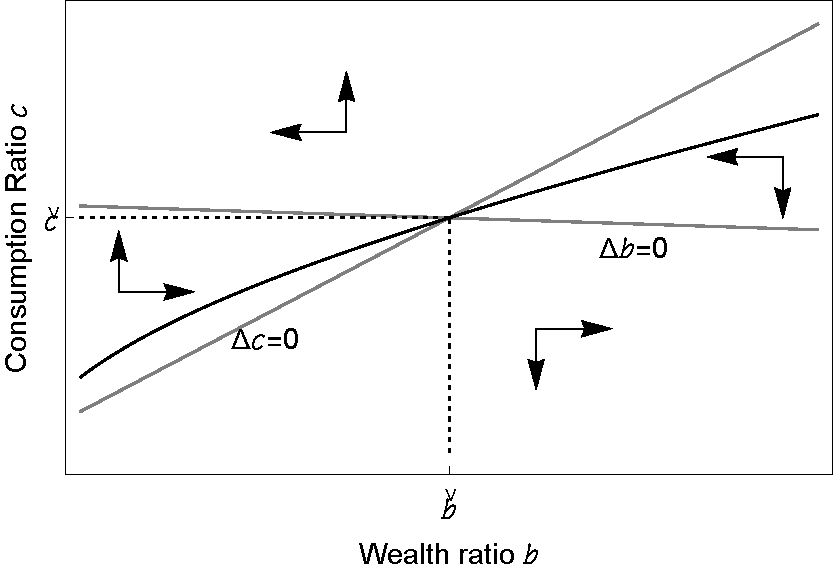
\includegraphics[width=.65\textwidth]{../figures/phaseDiag.pdf}
    \end{figure}
\end{frame}

%----------------------------------------------------------------------------------------------------------------------------------

\begin{frame}
\frametitle{The Growth Impatience Condition}
\begin{itemize}
    \item Target wealth-to-income ratio: impatience vs prudence.

    \item Closed-form solution for the target wealth-to-income ratio
\input ../equations/bTargE.tex
    \item \begin{eqnarray}
\frac{\partial \bTarg}{\partial \urate}>0,
\frac{\partial \bTarg}{\partial \beta}>0,
\frac{\partial \bTarg}{\partial \PGro}<0.
\label{eq:compstat}
\end{eqnarray}


\begin{eqnarray}
\frac{\partial \bTarg}{\partial \CRRA}>0.
\label{eq:db/drho=}
\end{eqnarray}
    \item The response of $\bTarg$ to $\Rfree$ is ambiguous. 
\end{itemize}
\end{frame}



%----------------------------------------------------------------------------------------------------------------------------------
\subsection{Foreign Assets}
\begin{frame}
\frametitle{Foreign Assets}
    \begin{itemize}
    \item Ratio of employed workers' wealth to output,
\input ../equations/BRatEIndAgg.tex
where $\LGro$ is the factor by which the share of a generation in total labor supply shrinks every period.

    \item The Level of Unemployed Workers' Wealth is 
\input ../equations/BLevUtp1.tex
\end{itemize}
\end{frame}

\begin{frame}\frametitle{Foreign Assets (cont)}
\begin{itemize}
\item Steady state ratio of net foreign assets to GDP
    \input ../equations/NFARat
\item Depends on Employed Workers' Target Savings
\end{itemize}
\end{frame}

\begin{frame}\frametitle{`Stakes'}
\begin{itemize}
    \item Model with no stakes
\input ../equations/BRatENostake
    \item Model with stakes yielding a representative agent
\input ../equations/BRatEStakes
\end{itemize}
where
\input ../equations/bTargEStakes

\end{frame}

\begin{frame}\frametitle{Advantages Of Model With Stakes}

\begin{itemize}
   \item Closed-form solution for steady state
   \item Simple to characterize transition dynamics
\end{itemize}

\end{frame}



%----------------------------------------------------------------------------------------------------------------------------------
\section{Calibration And Simulation}
\subsection{Parameter Values}
\begin{frame}
\frametitle{Calibration and Simulation}


\centerline{\bf Table 1}

\begin{center}
\begin{tabular}{|c|c|c|c|c|c|c|c|c|c|}
  \hline
  % after \\: \hline or \cline{col1-col2} \cline{col3-col4} ...
  $\kapShare$ & $\delta$ & $\PopGro$ & $\WGro$ & $\Rfree$ & $\beta^{-1}$ & $\PtyGro$ & $\urate$ & $\CRRA$ & $\pDies$ \\ \hline
  0.3 & 0.06 & 1.01 & 1.04 & 1.04 & 1.04 & 1.01 & 0.025 & 2 & 0.05 \\
  \hline
\end{tabular}
\end{center}

    \begin{itemize}
    \item ${\NFALev}/{\GDPLev}=0.17$ in the model with no stakes
    \item ${\NFALev}/{\GDPLev}=0.79$ in the model with stakes
    \end{itemize}

\end{frame}

\subsection{Paths}
%----------------------------------------------------------------------------------------------------------------------------------
\begin{frame}
\frametitle{Paths}
    \begin{figure}
    \centering
    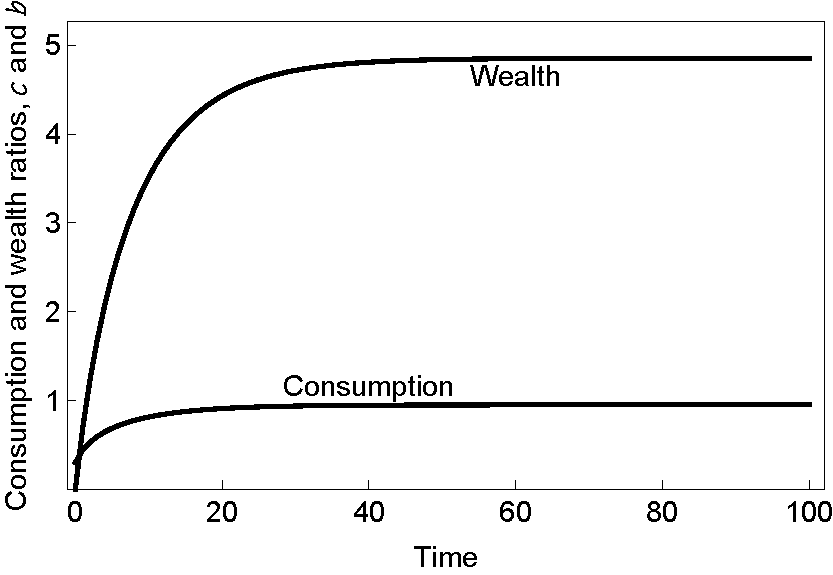
\includegraphics[width=.6\textwidth]{../figures/paths.pdf}
    \end{figure}
  \end{frame}

%----------------------------------------------------------------------------------------------------------------------------------
\subsection{Sensitivity Analysis}

\begin{frame}
\frametitle{Sensitivity analysis}
    \begin{figure}
    \centering
    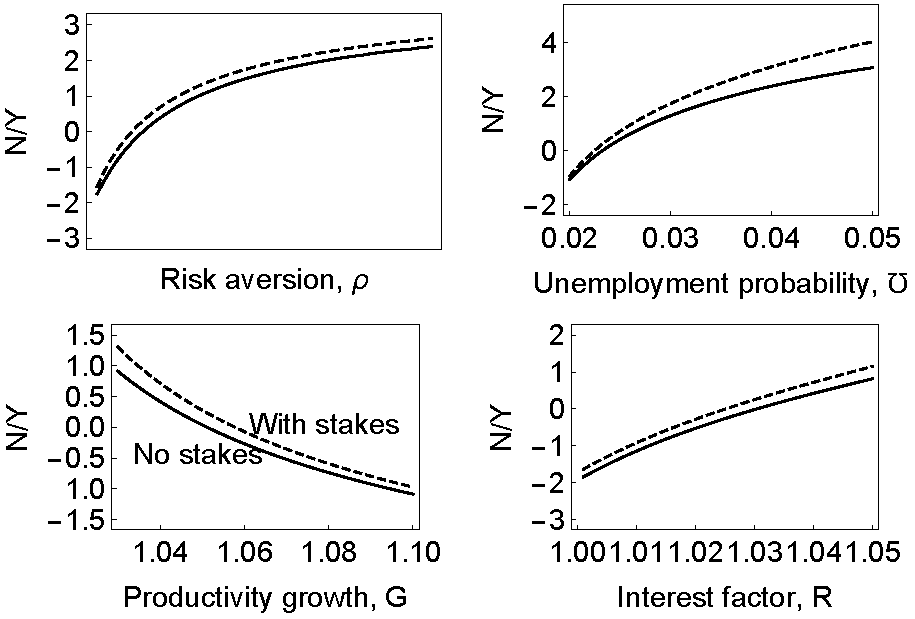
\includegraphics[width=.6\textwidth]{../figures/sensitivity.pdf}
    \end{figure}
\end{frame}

%----------------------------------------------------------------------------------------------------------------------------------

\subsection{Social Insurance}
\begin{frame}
\frametitle{Social Insurance}
    \begin{itemize}
    \item Many countries have social transfers to unemployed/retired
    \item New assumption: labor income tax on the employed in order to finance transfers to
the unemployed.
    \item Unemployed receive transfer whose value is a multiple $\Severance$ of the labor income that they would have received if they had remained employed.
    \item New formula for target wealth-to-income ratio.  Going through the same steps as before, we get
\input ../equations/bTargWithSocIns
%
%\begin{eqnarray}
%\bTarg(\Severance) = \bTarg 
%\left[1-\Severance \left(\frac{\urate \PtyGro}{\PopGro}+\MPC %\left(1+\frac{\PatPGro^{-\CRRA}-1}{\urate}\right)^{1/\CRRA}\right)\right],
%\end{eqnarray}
    \end{itemize}

\end{frame}

%----------------------------------------------------------------------------------------------------------------------------------

\begin{frame}
\frametitle{Social insurance}
    \begin{figure}
    \centering
    \includegraphics[width=.6\textwidth]{../figures/socins.pdf}
    \end{figure}
\end{frame}

%----------------------------------------------------------------------------------------------------------------------------------

\section{Applications}
\subsection{Growth And Saving}
\begin{frame}
\frametitle{Growth And Saving}
    \begin{itemize}
    \item Theory: Good Growth Prospects $\rightarrow$ Should Borrow to Invest
    \item Data: Fast-Growing Countries {\it Export} Capital 
\begin{itemize}
\item \cite{carroll&weil:crcs}; \cite{lss:whatdrives}; \cite{aps:sgi}; Gourinchas and Jeanne, 2007, Prasad, Rajan and Subramanian (2007); Sandri (2008)
\end{itemize}
    \item Can this model shed light on this puzzle?
    \item Yes, if growth take-off entails idiosyncratic risk (both $\WGro$ and $\urate$ go up).
    \end{itemize}

\end{frame}

%----------------------------------------------------------------------------------------------------------------------------------

\begin{frame}
\frametitle{Growth and capital flows}
    \begin{figure}
    \centering
    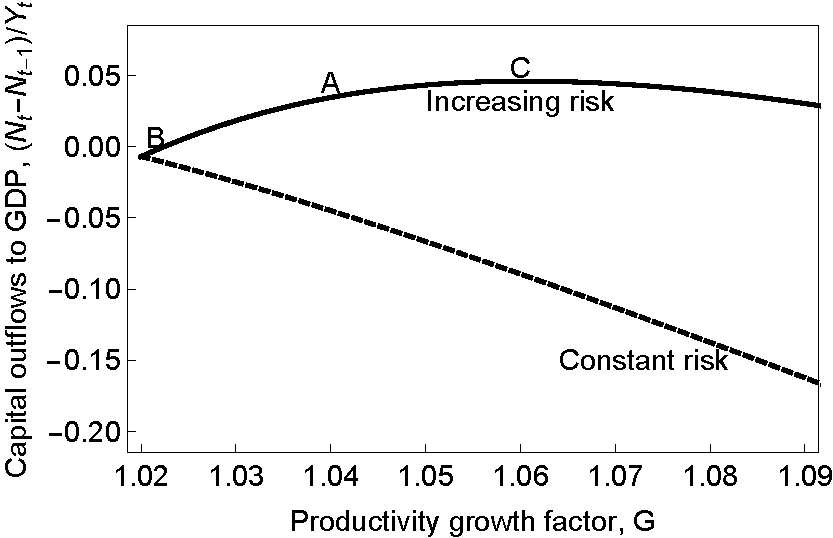
\includegraphics[width=.6\textwidth]{../figures/capOutflows.pdf}
    \end{figure}
\end{frame}

%----------------------------------------------------------------------------------------------------------------------------------
\subsection{Resorbing Global Imbalances}
\begin{frame}
\frametitle{World General Equilibrium}
    \begin{itemize}
    \item Small economy assumption not appropriate to study global savings glut or adjustment of global financial imbalances. 
    \item Study steady state equilibria in two-country extension of the model.
    \item Global interest rate $\Rfree$ endogenous
\begin{eqnarray}
\NFALev_h+\NFALev_f=0,
\end{eqnarray}
    \end{itemize}

\end{frame}

%----------------------------------------------------------------------------------------------------------------------------------
\begin{frame}
\frametitle{General Equilibrium}
    \begin{itemize}
    \item Two countries identical except for size (h=20\%, f=80\%) and level of social insurance ($\Severance_h=1.5$, $\Severance_f=0.75$).
    \item This implies
    \begin{eqnarray}
    \frac{\NFALev_h}{\GDPLev_h}&=&-0.5 \\
    \frac{\NFALev_f}{\GDPLev_f}&=&0.125
    \end{eqnarray}
    \item What is impact of increasing foreign social insurance to the home level?
    \end{itemize}
\end{frame}

%----------------------------------------------------------------------------------------------------------------------------------

\begin{frame}
\frametitle{General equilibrium}
    \begin{figure}
    \centering
    \includegraphics[width=.55\textwidth]{../figures/geneqbm.pdf}
    \end{figure}
\end{frame}

%----------------------------------------------------------------------------------------------------------------------------------
\section{Conclusions}

\begin{frame}
\frametitle{Conclusions}
    \begin{itemize}
    \item Tractable model of net foreign assets of small open economy
    \item Two applications
        \begin{itemize}
        \item Relationship between growth and capital flows
        \item Long-run implications of reducing global imbalances.
        \end{itemize}
    \item Extensions for future research: portfolio choice, real exchange rates, asset prices, etc.
    \end{itemize}

\end{frame}

\tiny 
\beamerdefaultoverlayspecification{<*>}

\begin{frame}[allowframebreaks]
\frametitle{\textbf{References}}
\tiny
\input bibMake
\end{frame}

\end{document} 
